\chapter{系统设计}

\setlength{\textfloatsep}{10pt plus 2pt minus 2pt}
\setlength{\floatsep}{10pt plus 2pt minus 2pt}
\setlength{\intextsep}{10pt plus 2pt minus 2pt}
\setlength{\abovecaptionskip}{4pt}
\setlength{\belowcaptionskip}{0pt}
\renewcommand{\topfraction}{0.9}
\renewcommand{\bottomfraction}{0.8}
\renewcommand{\textfraction}{0.08}
\renewcommand{\floatpagefraction}{0.8}

本章在第三章需求分析的基础上，结合当前前后端代码与数据库脚本，对系统的整体架构、功能模块、数据库、安全控制和界面原型进行设计说明。系统设计的目标不是重新描述需求，而是说明这些需求如何被组织为可实现、可扩展和可维护的软件结构。

\section{总体架构设计}
\subsection{系统层次结构图}
本系统采用前后端分离的 B/S 结构。在这一结构下，系统被划分为表现层、业务层和数据层。表现层面向用户交互，主要包括登录页、生成工作台、历史版本页、用户管理页，以及路由、状态管理、请求封装和预览沙箱等前端基础能力。业务层面向业务处理，主要包括认证鉴权、项目与工作区管理、生成任务编排、版本管理、成本控制、安全扫描和审计服务等后端组件。数据层面向持久化存储，主要包括用户、会话、工作区、项目、任务、版本、调用日志和审计日志等数据对象。

从代码实现看，表现层由 Vue 3、Vue Router、Pinia 和 Element Plus 共同支撑，页面入口集中在 \texttt{GeneratorView}、\texttt{HistoryView}、\texttt{LoginView} 和 \texttt{AdminUsersView}。业务层由 Spring Boot 单体应用承载，控制器负责资源入口，服务层负责业务编排，仓储层负责实体持久化。数据层由 MySQL 和 JPA Repository 组成，用于承载上述核心业务数据。这样的分层方式使各层关注点保持清晰，便于后续维护和扩展（Architectural Styles and the Design of Network-based Software Architectures）\cite{fielding2000rest}。

图 \ref{fig:chapter4-layer-architecture} 主要展示三层结构中分别包含哪些内容。表现层集中展示前端页面与状态管理组件，业务层集中展示控制器、服务和通用处理组件，数据层集中展示持久化表和仓储对象。该图的重点不在于描述详细调用顺序，而在于说明系统按层组织后的组成边界。

\begin{figure}[!htbp]
\centering
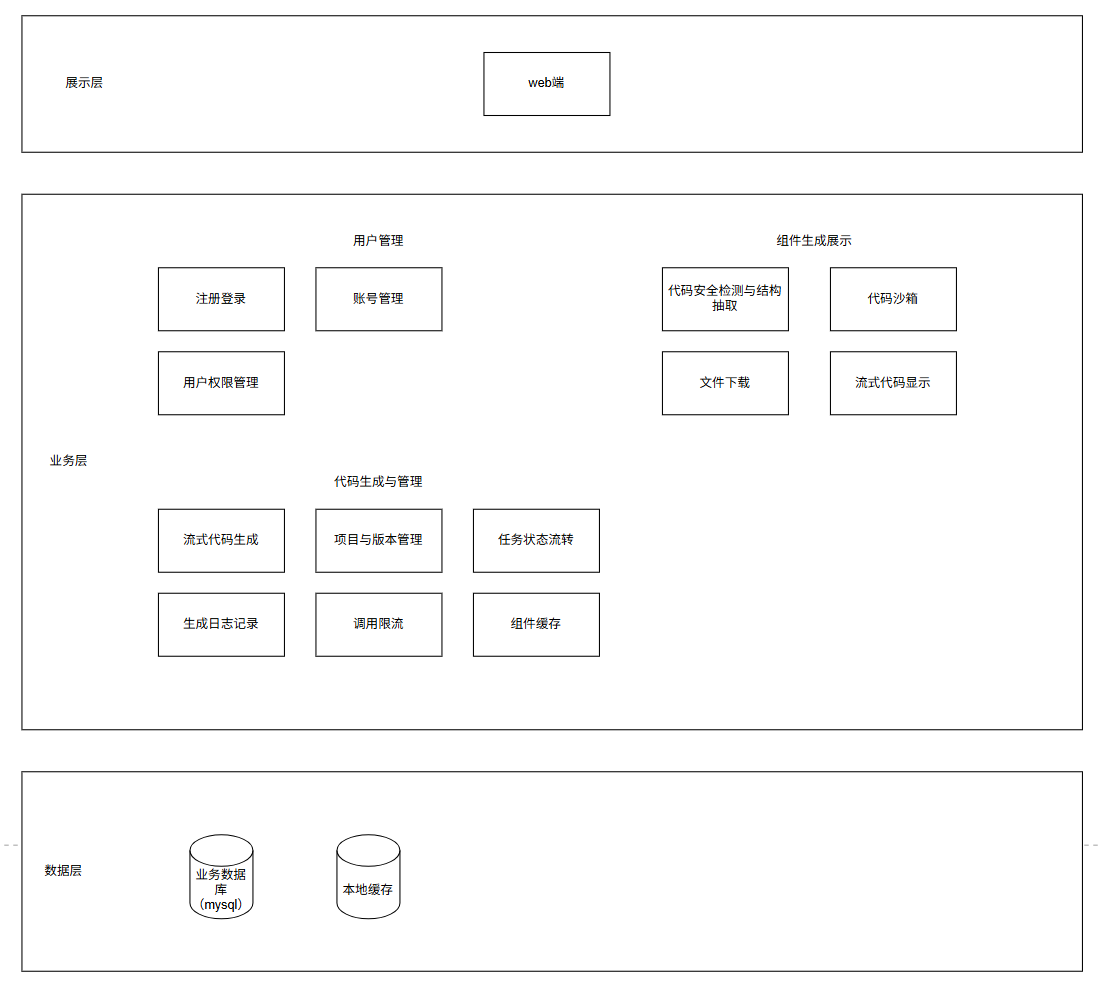
\includegraphics[width=0.96\textwidth,height=0.48\textheight,keepaspectratio]{figures/系统层次结构图.png}
\caption{系统层次结构图}
\label{fig:chapter4-layer-architecture}
\end{figure}

\subsection{技术架构图}
技术架构图用于说明项目从接受请求到完成处理的链路，以及链路中各组件之间如何协同工作。当前系统的请求入口位于浏览器端。前端在用户提交登录、项目切换或组件生成请求后，通过统一请求封装附加 \texttt{X-Auth-Token} 与 \texttt{X-Project-Id} 请求头，再将请求发送到后端控制器。控制器接收请求后，先完成身份校验和资源归属校验，再根据请求类型进入会话处理、项目处理或生成任务处理流程。

对于组件生成场景，系统的处理链路更为完整。后端在接收请求后先创建任务记录，再建立 SSE 流式连接，将任务开始、token 输出、异常信息和完成状态逐步返回前端。生成过程中，\texttt{GenerationStreamService} 负责组织任务状态流转，\texttt{QwenLlmClient} 负责调用模型服务，\texttt{SfcCodeExtractor} 负责提取结构化代码，\texttt{CodeSafetyScanner} 负责执行安全检查，最后由版本服务和日志服务完成结果入库。前端接收到最终结果后，再更新代码面板、预览面板和历史记录。接口组织上，系统采用资源路径和 HTTP 动词表达不同业务入口，生成流单独使用 SSE，以支持长耗时任务的持续回传（Architectural Styles and the Design of Network-based Software Architectures）（Server-Sent Events）\cite{fielding2000rest}\cite{w3c_eventsource}。

图 \ref{fig:chapter4-tech-architecture} 主要展示请求从进入系统到处理完成的顺序，以及浏览器、前端状态层、控制器、认证组件、任务服务、模型接入组件、解析与安全组件、数据库之间的交互关系。该图的重点不在于分层归类，而在于说明请求处理链路和关键组件之间的调用关系。

\begin{figure}[!htbp]
\centering
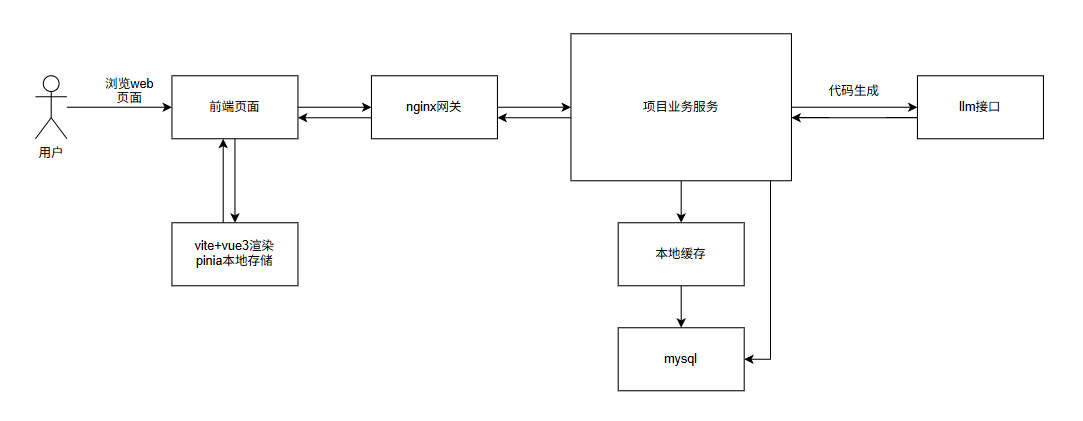
\includegraphics[width=0.96\textwidth,height=0.50\textheight,keepaspectratio]{figures/技术架构图.png}
\caption{技术架构图}
\label{fig:chapter4-tech-architecture}
\end{figure}

\section{功能模块设计}
\subsection{模块划分}
结合前后端代码，系统可以划分为账号与权限、项目与工作区、组件生成、版本管理、成本控制、管理员治理、在线预览与下载七个模块。这样的划分是依据业务边界而不是代码文件数量确定的。每个模块都围绕明确的数据对象和交互入口组织，便于后续迭代时定位影响范围。

账号与权限模块负责建立会话身份并约束接口访问边界，是后续业务调用的前提。项目与工作区模块负责组织用户的任务归属关系，保证生成记录、版本记录和下载操作都在正确的项目范围内执行。组件生成模块负责接收需求、编排任务、调用模型并产出代码，是系统的核心处理模块。版本管理模块负责保存历史结果并提供回看、对比和下载入口。成本控制模块负责统计 token 使用量、估算费用并执行限流策略。管理员治理模块负责用户检索、角色调整、账号启停和审计记录查询。在线预览与下载模块负责对生成结果进行结构化拆分、安全检测、运行时渲染和文件导出。

图 \ref{fig:chapter4-module-interaction} 给出了模块之间的协作关系。前端模块并不直接操作数据库，它们统一通过资源接口与后端交互；后端模块之间则围绕任务、版本和用户上下文完成服务调用。生成模块是整个系统的中心模块，项目上下文、权限校验、版本保存和成本记录都会在该模块周围发生。

各模块的前端入口、后端组件和职责划分见表 \ref{tab:chapter4-module-split}。

\begin{figure}[!htbp]
\centering
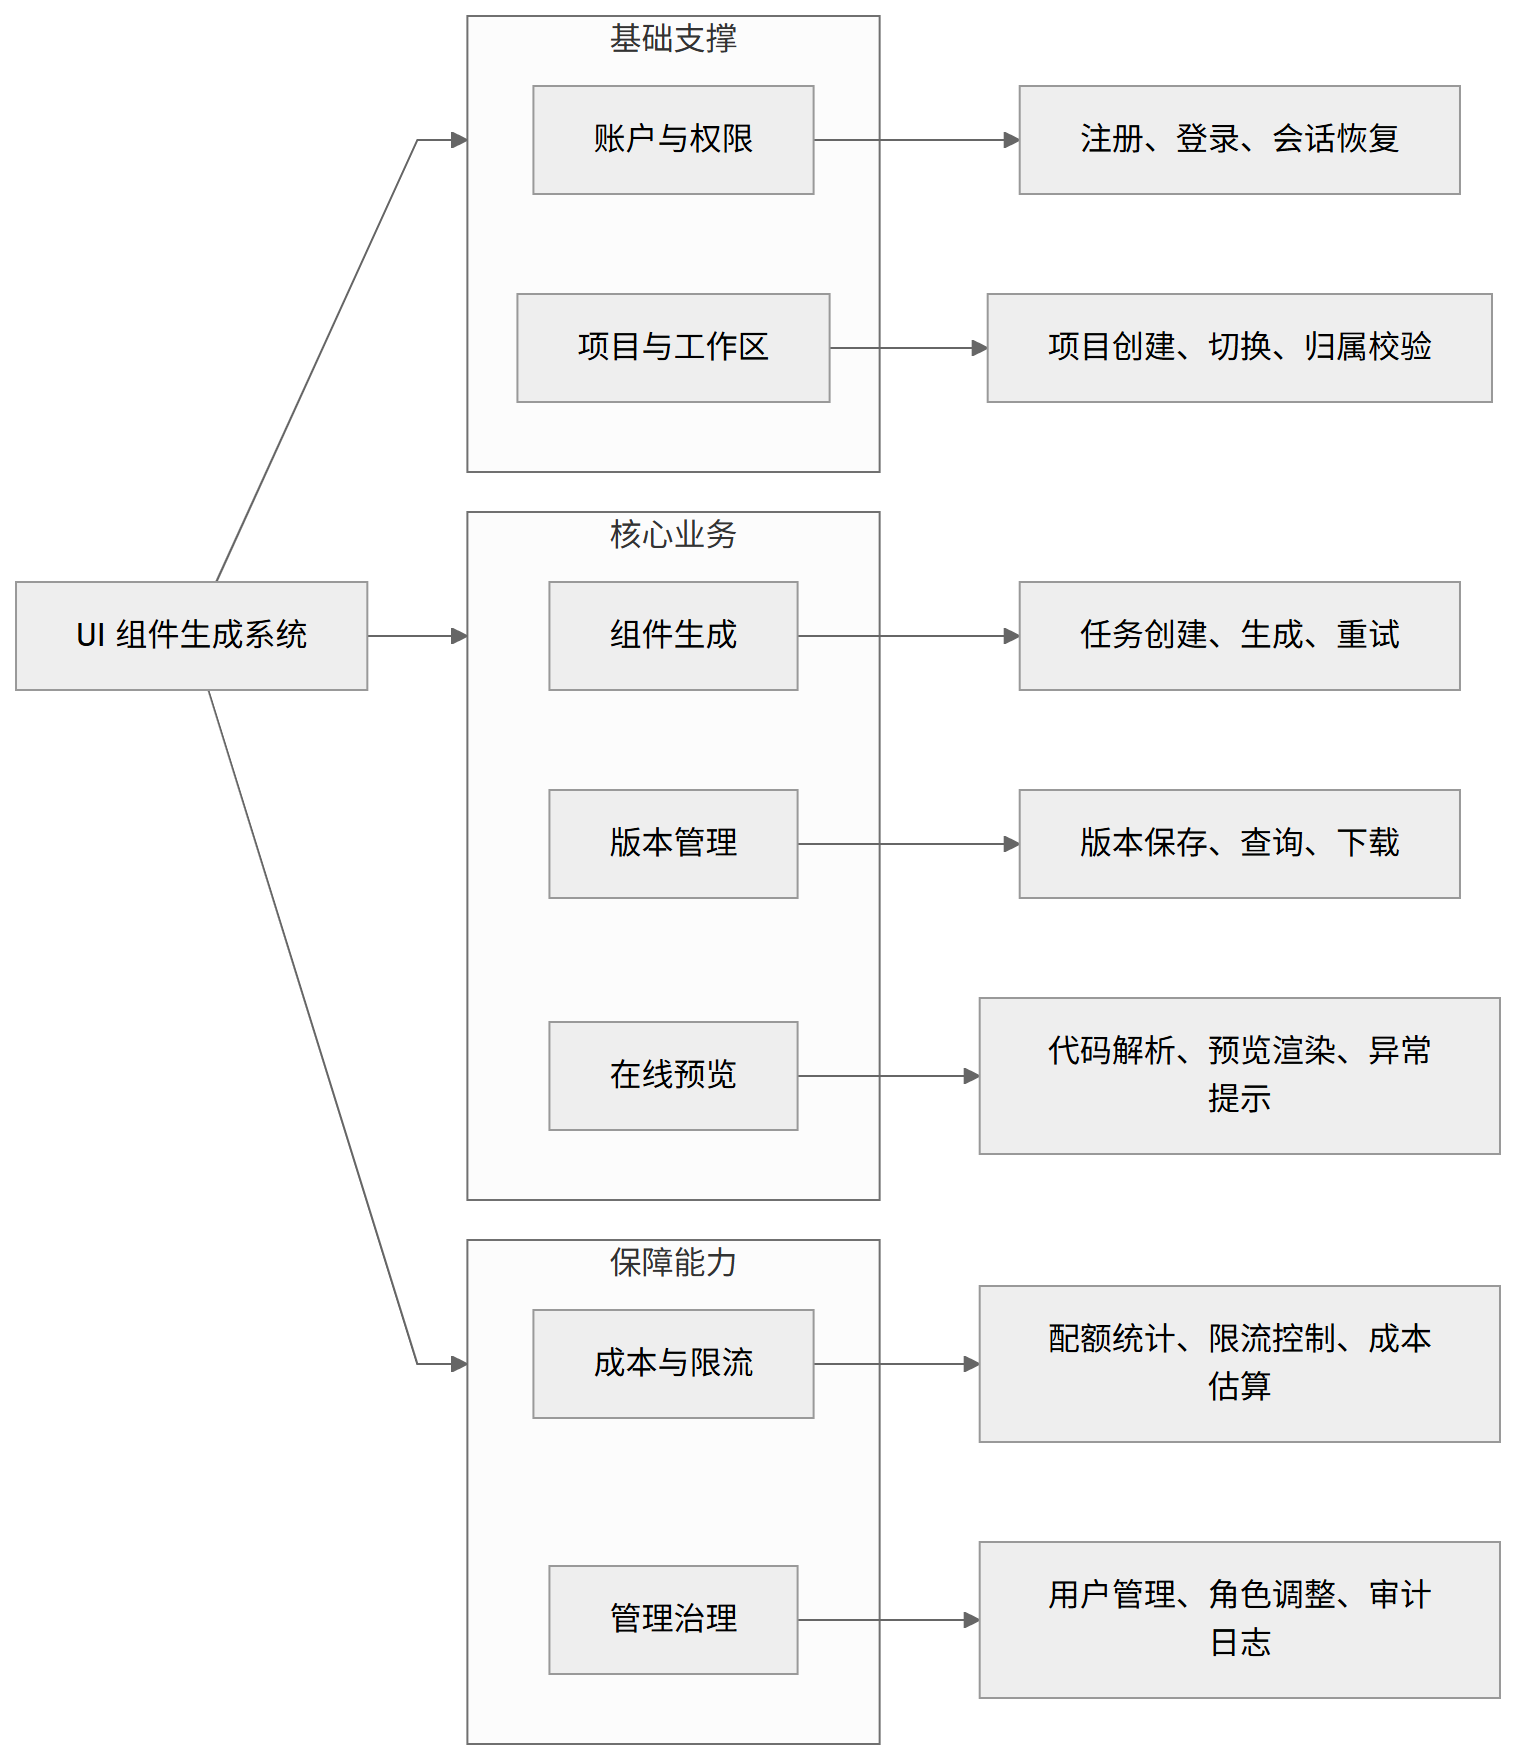
\includegraphics[width=0.96\textwidth,height=0.46\textheight,keepaspectratio]{figures/functional-modules.png}
\caption{核心功能模块关系图}
\label{fig:chapter4-module-interaction}
\end{figure}

\begin{table}[!htbp]
\centering
\caption{功能模块划分与职责}
\label{tab:chapter4-module-split}
\small
\begin{tabular}{@{}p{0.17\textwidth}p{0.22\textwidth}p{0.17\textwidth}p{0.32\textwidth}@{}}
\toprule
模块名称 & 前端入口 & 后端核心组件 & 主要职责 \\
\midrule
账号与权限模块 & 登录页、导航守卫 & 认证入口、会话服务、权限校验 & 完成注册、登录、登出、用户信息恢复、角色识别和权限校验 \\
项目与工作区模块 & 顶部项目切换、项目创建对话框 & 项目服务、工作区服务 & 创建项目、分配工作区、维护当前项目上下文，保证任务只能在所属项目内执行 \\
组件生成模块 & 生成工作台 & 任务服务、流式生成服务、模型接入组件 & 创建任务、建立流式连接、调用模型、维护任务状态、生成组件代码 \\
版本管理模块 & 历史页、下载按钮 & 版本控制器、版本服务 & 查询任务历史版本、返回版本详情、下载指定版本文件、统计下载次数 \\
成本控制模块 & 顶部 token 用量标签 & 用量统计服务、限流组件 & 统计当日 token 使用量、估算费用、执行配额校验和频率限制 \\
管理员治理模块 & 用户管理页 & 管理接口、审计服务 & 查询用户、调整角色、启停账号、查询审计日志 \\
在线预览与下载模块 & 代码面板、预览面板、下载入口 & 预览沙箱、结构提取、安全扫描 & 对生成结果进行结构化处理、安全检测、运行时预览和文件下载 \\
\bottomrule
\end{tabular}
\end{table}

\subsection{模块间接口设计}
模块之间的接口分为两类。一类是前端与后端之间的 HTTP/SSE 接口，这部分决定了页面能否获得正确数据和实时反馈。另一类是后端内部服务接口，这部分决定了任务执行链路能否保持一致。前者关注请求参数、返回结构和资源边界，后者关注任务状态、事务边界和异常传播。

在前后端接口设计上，系统将资源路径统一挂载在 \texttt{/api/v1} 下。普通查询与变更接口采用 JSON 返回，生成任务的执行过程采用 SSE 返回 \texttt{started}、\texttt{token}、\texttt{final\_code}、\texttt{error} 和 \texttt{done} 等事件。这样既能保持接口风格一致，也能为长耗时生成任务提供连续的状态回传（Server-Sent Events）\cite{w3c_eventsource}。

主要外部接口的输入与输出关系见表 \ref{tab:chapter4-api-design}。

\begin{table}[!htbp]
\centering
\caption{主要外部接口设计}
\label{tab:chapter4-api-design}
\small
\begin{tabular}{@{}p{0.15\textwidth}p{0.13\textwidth}p{0.24\textwidth}p{0.34\textwidth}@{}}
\toprule
接口分组 & 方法 & 关键输入 & 主要输出 \\
\midrule
认证接口 & \texttt{POST} / \texttt{GET} & 用户名、密码、认证令牌 & 会话令牌、用户编号、用户角色、过期时间、当前用户信息 \\
项目接口 & \texttt{POST} / \texttt{GET} & 项目名称、描述、当前登录态 & 项目编号、项目名称、工作区标识、项目列表 \\
任务创建接口 & \texttt{POST} & 工作区标识、项目编号、组件名称、需求描述、约束 JSON、演示数据开关 & 任务编号、任务状态 \\
生成流接口 & \texttt{GET} (SSE) & 工作区标识、项目编号、任务编号 & 流式 token、最终代码、错误事件、完成状态 \\
历史任务接口 & \texttt{GET} & 项目编号、分页参数 & 任务摘要列表、总记录数、分页信息 \\
版本详情接口 & \texttt{GET} & 工作区标识、项目编号、版本编号 & 版本详情、\texttt{vue\_code}、安全级别、结构完整性标记 \\
版本下载接口 & \texttt{GET} & 工作区标识、项目编号、版本编号 & Vue 单文件组件下载流 \\
用量接口 & \texttt{GET} & 当前用户身份 & 每日配额、已用 token、剩余额度、估算费用 \\
管理接口 & \texttt{GET} / \texttt{PATCH} & 关键字、用户编号、目标角色、启停状态 & 用户摘要、角色变更结果、账号状态变更结果、审计日志分页数据 \\
\bottomrule
\end{tabular}
\end{table}

后端内部服务接口围绕任务生命周期展开。生成模块接收请求后，\texttt{GenerationService} 先创建任务记录并校验项目归属；\texttt{GenerationStreamService} 再负责状态迁移、模型调用、代码抽取、安全检查和版本持久化；\texttt{ComponentVersionService} 负责版本详情和下载出口；\texttt{CostControlService} 负责配额判断与调用成本累计。模块之间虽然是方法调用关系，但都以任务编号、项目编号和用户上下文为连接点，因此任务链路具有明确的状态边界。

\section{数据库设计}
\subsection{E-R 图}
数据库设计围绕用户、项目、任务和版本展开。系统当前包含 \texttt{app\_user}、\texttt{user\_session}、\texttt{workspace}、\texttt{project\_space}、\texttt{generation\_task}、\texttt{component\_version}、\texttt{llm\_call\_log} 和 \texttt{audit\_log} 八个核心实体。用户与会话是一对多关系，用户与项目是一对多关系，项目与工作区在当前实现中是一对一关系，项目与任务是一对多关系，任务与版本、调用日志也是一对多关系。

图 \ref{fig:chapter4-er} 展示了主要实体及其关系。其中，\texttt{project\_space} 通过 \texttt{workspace\_id} 绑定唯一工作区。任务表同时保留 \texttt{project\_id} 与 \texttt{workspace\_id}，用来区分项目范围和执行上下文。这样的设计使任务既可以验证项目归属，也可以校验工作区来源。调用日志和审计日志不直接参与主业务流程输出，但它们对于成本统计和管理追踪是必要的。

\begin{figure}[!htbp]
\centering
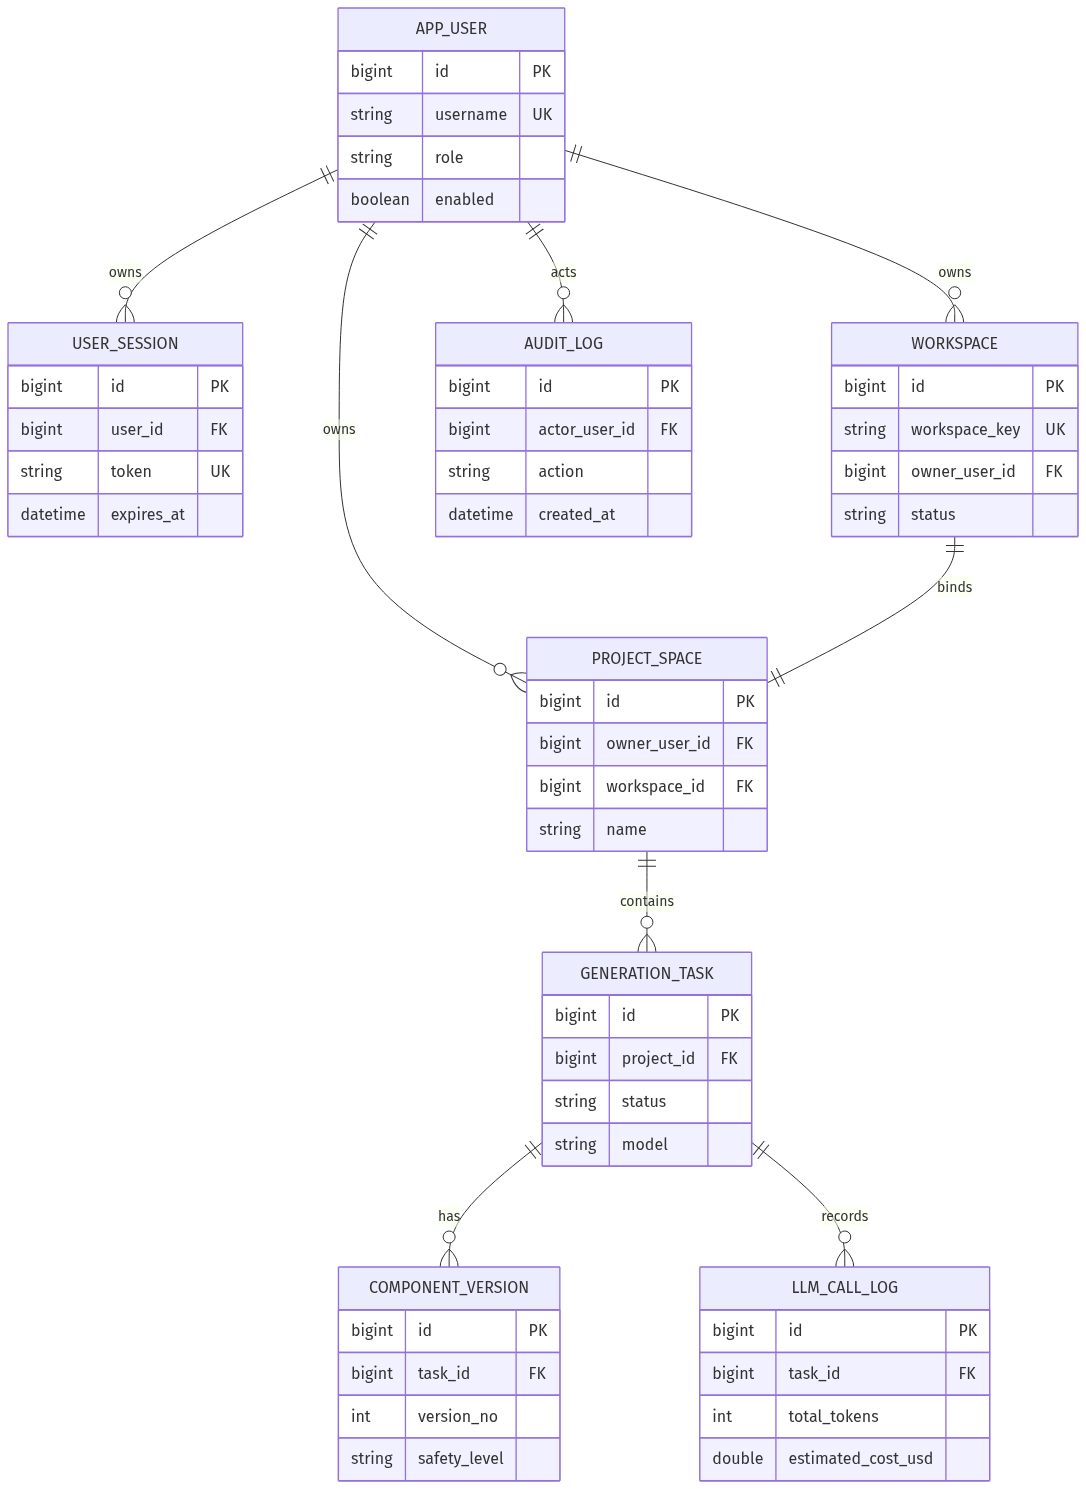
\includegraphics[width=0.94\textwidth,height=0.58\textheight,keepaspectratio]{figures/chapter3-er-mermaid.png}
\caption{系统 E-R 图}
\label{fig:chapter4-er}
\end{figure}

\subsection{数据表结构设计}
本系统的数据表设计强调“一个业务对象对应一类记录”的原则。账号、项目、任务、版本和治理信息分别落到独立数据表中，避免在单表中混杂过多职责。表结构中保留了足够的时间字段，便于完成列表排序、历史回看和审计追踪。

账号、项目相关数据表见表 \ref{tab:chapter4-db-user-project}，生成与治理相关数据表见表 \ref{tab:chapter4-db-generation}。

\begin{table}[!htbp]
\centering
\caption{账号与项目域数据表设计}
\label{tab:chapter4-db-user-project}
\small
\begin{tabular}{@{}p{0.18\textwidth}p{0.30\textwidth}p{0.38\textwidth}@{}}
\toprule
表名 & 主要字段 & 设计说明 \\
\midrule
\texttt{app\_user} & \texttt{id}、\texttt{username}、\texttt{password\_hash}、\texttt{role} & 存储用户基本身份、口令哈希和角色状态，是认证授权的主表 \\
\texttt{user\_session} & \texttt{id}、\texttt{user\_id}、\texttt{token}、\texttt{expires\_at} & 存储服务端会话令牌及有效期，用于恢复当前登录用户 \\
\texttt{workspace} & \texttt{id}、\texttt{workspace\_key}、\texttt{owner\_user\_id}、\texttt{status} & 记录工作区上下文。匿名工作区与登录后项目工作区都基于该表管理 \\
\texttt{project\_space} & \texttt{id}、\texttt{owner\_user\_id}、\texttt{workspace\_id}、\texttt{name} & 表示用户项目空间，绑定唯一工作区，所有任务与版本都归属于具体项目 \\
\bottomrule
\end{tabular}
\end{table}

\begin{table}[!htbp]
\centering
\caption{生成与治理域数据表设计}
\label{tab:chapter4-db-generation}
\small
\begin{tabular}{@{}p{0.18\textwidth}p{0.30\textwidth}p{0.38\textwidth}@{}}
\toprule
表名 & 主要字段 & 设计说明 \\
\midrule
\texttt{generation\_task} & \texttt{id}、\texttt{project\_id}、\texttt{prompt}、\texttt{component\_name}、\texttt{status} & 记录每次生成请求及其状态，是任务编排与历史查询的核心表 \\
\texttt{component\_version} & \texttt{id}、\texttt{task\_id}、\texttt{version\_no}、\texttt{vue\_code}、\texttt{safety\_level} & 保存任务产出的每个版本；\texttt{compile\_ok} 用于表示结构完整性标记，而不是调用真实编译器后的结果 \\
\texttt{llm\_call\_log} & \texttt{id}、\texttt{task\_id}、\texttt{provider}、\texttt{request\_tokens}、\texttt{estimated\_cost\_usd} & 记录模型调用消耗和耗时，用于成本控制与问题追踪 \\
\texttt{audit\_log} & \texttt{id}、\texttt{actor\_user\_id}、\texttt{target\_user\_id}、\texttt{action} & 记录管理员操作，支撑角色调整和账号启停的事后审计 \\
\bottomrule
\end{tabular}
\end{table}

字段设计中，\texttt{prompt}、\texttt{constraints\_json} 和 \texttt{vue\_code} 等内容采用长文本存储，因为这些字段长度波动较大；状态、角色和安全级别采用枚举字符串存储，以便代码和数据库保持一致的可读性；所有业务主表都保留创建时间和更新时间，为排序、缓存刷新和审计查询提供依据。

\subsection{索引设计与优化}
索引设计直接依据当前代码中的查询路径确定。任务列表按项目和创建时间倒序查询，版本列表按任务和版本号查询，项目列表按拥有者和更新时间查询，审计日志按时间倒序查询，因此这些字段被放在联合索引或单列索引中。索引设计应服务于主要访问路径，而不是为所有字段都建立索引（MySQL 8.0 Reference Manual）\cite{mysqldocs2025}。

主要数据表的索引字段与适用场景见表 \ref{tab:chapter4-index-design}。

\begin{table}[!htbp]
\centering
\caption{主要数据表索引设计}
\label{tab:chapter4-index-design}
\footnotesize
\begin{tabular}{@{}p{0.19\textwidth}p{0.18\textwidth}p{0.22\textwidth}p{0.25\textwidth}@{}}
\toprule
表名 & 索引或约束名称 & 索引字段 & 作用场景 \\
\midrule
\texttt{app\_user} & 用户名唯一索引 & \texttt{username} & 支撑登录时按用户名定位用户，并保证用户名不重复 \\
\texttt{user\_session} & 会话令牌唯一索引 & \texttt{token} & 支撑拦截器按令牌恢复当前会话，避免重复令牌 \\
\texttt{user\_session} & 用户会话索引 & \texttt{user\_id, expires\_at} & 支撑查询用户会话和清理过期会话 \\
\texttt{workspace} & 工作区键唯一索引 & \texttt{workspace\_key} & 支撑按工作区标识恢复上下文，避免工作区键重复 \\
\texttt{project\_space} & 项目拥有者索引 & \texttt{owner\_user\_id, updated\_at} & 支撑按用户加载项目列表和最近项目优先展示 \\
\texttt{project\_space} & 工作区唯一约束 & \texttt{workspace\_id} & 保证一个工作区只绑定一个项目空间 \\
\texttt{generation\_task} & 任务项目索引 & \texttt{project\_id, created\_at} & 支撑历史页按项目分页查询任务列表 \\
\texttt{generation\_task} & 任务工作区索引 & \texttt{workspace\_id, created\_at} & 支撑按工作区查看任务记录和最近生成排序 \\
\texttt{component\_version} & 版本任务索引 & \texttt{task\_id, created\_at} & 支撑同一任务下版本倒序展示 \\
\texttt{component\_version} & 任务版本唯一约束 & \texttt{task\_id, version\_no} & 保证同一任务的版本号唯一，防止重复版本编号 \\
\texttt{llm\_call\_log} & 模型调用任务索引 & \texttt{task\_id, created\_at} & 支撑按任务查看模型调用记录和成本信息 \\
\texttt{audit\_log} & 审计操作人索引 & \texttt{actor\_user\_id, created\_at} & 支撑按操作人查看审计记录 \\
\texttt{audit\_log} & 审计时间索引 & \texttt{created\_at} & 支撑管理员按时间倒序查看最近审计日志 \\
\bottomrule
\end{tabular}
\end{table}

在优化策略上，系统没有对长文本字段建立索引，因为这些字段主要用于保存内容，不用于高频过滤。版本下载次数字段也未单独建索引，因为它主要承担统计功能，不参与主查询条件。当前索引方案已经覆盖了历史页、项目页和管理页的主要访问路径，能够满足现阶段单体系统的查询需求。

\section{安全设计}
\subsection{身份认证机制}
本系统没有采用无状态 JWT，而是采用服务端会话令牌机制。用户注册或登录成功后，\texttt{AuthService} 生成随机令牌，写入 \texttt{user\_session} 表，并将令牌返回给前端。前端在后续请求中通过 \texttt{X-Auth-Token} 请求头携带令牌，\texttt{AuthInterceptor} 在进入控制器之前完成令牌校验，并把当前用户写入 \texttt{AuthContextHolder}，供服务层继续使用。

这种认证方式与当前项目的实现边界更匹配，因为系统需要在服务端控制会话过期、用户禁用和管理员审计。若用户被禁用或令牌过期，后端可以直接阻断访问。角色和权限校验由 \texttt{AuthorizationService} 完成，管理员能力通过 \texttt{USER\_MANAGE} 和 \texttt{AUDIT\_READ} 两类权限映射到 \texttt{ADMIN} 角色上。分级访问与最小权限控制属于后台管理系统的基本安全要求（GB/T 22239-2019 信息安全技术 网络安全等级保护基本要求）\cite{gbt22239_2019}。

身份认证的主要处理步骤见表 \ref{tab:chapter4-auth-flow}。

\begin{table}[!htbp]
\centering
\caption{身份认证处理流程}
\label{tab:chapter4-auth-flow}
\small
\begin{tabular}{@{}p{0.15\textwidth}p{0.27\textwidth}p{0.46\textwidth}@{}}
\toprule
阶段 & 处理组件 & 处理内容 \\
\midrule
登录提交 & \texttt{AuthController} & 接收用户名和密码，调用认证服务 \\
口令校验 & \texttt{AuthService} & 使用 BCrypt 校验口令哈希，检查账号是否启用 \\
会话生成 & \texttt{AuthService}、\texttt{user\_session} & 生成随机令牌，写入过期时间和最后活跃时间 \\
请求拦截 & \texttt{AuthInterceptor} & 从请求头读取 \texttt{X-Auth-Token}，恢复当前用户上下文 \\
权限控制 & \texttt{AuthorizationService} & 根据当前角色判断是否允许访问管理接口 \\
\bottomrule
\end{tabular}
\end{table}

\subsection{敏感数据保护方案}
敏感数据保护在本系统中包含账号口令、会话令牌、项目数据、模型调用数据和生成代码五类对象。口令不以明文形式保存，数据库中只存储 BCrypt 哈希；会话令牌由安全随机数生成并设置有效期；项目、任务和版本接口都依赖当前用户和项目编号进行归属校验；模型调用密钥只在后端配置中使用，不直接暴露给浏览器；生成代码在落库前和预览前分别执行安全检测。

后端安全扫描由 \texttt{CodeSafetyScanner} 完成，重点拦截 \texttt{eval}、\texttt{new Function}、远程脚本标签、远程导入和网络请求等高风险模式。前端的 \texttt{detectUnsafeCode} 会在预览前再次执行类似检测，并将样式限制在 \texttt{preview-host} 容器中，避免生成代码直接影响整页样式。对于 Web 系统而言，输入边界控制、口令保护、权限隔离和审计留痕属于基础控制项（OWASP Top 10: The Ten Most Critical Web Application Security Risks）（Secure Software Development Framework (SSDF) Version 1.1）\cite{owasp2021top10}\cite{nistssdf2024}。

系统还对工作区中记录的 \texttt{ip\_hash} 和 \texttt{ua\_hash} 采用哈希化处理，而不是直接保存明文来源信息。这种做法能够保留一定的追踪能力，同时减少原始识别信息暴露范围，符合最小化处理原则（GB/T 35273-2020 信息安全技术 个人信息安全规范）\cite{gbt35273_2020}。

敏感数据保护对象、风险点与控制方式见表 \ref{tab:chapter4-security-design}。

\begin{table}[!htbp]
\centering
\caption{敏感数据保护与安全控制}
\label{tab:chapter4-security-design}
\small
\begin{tabular}{@{}p{0.18\textwidth}p{0.28\textwidth}p{0.38\textwidth}@{}}
\toprule
保护对象 & 风险点 & 当前控制方式 \\
\midrule
用户口令 & 明文泄露、弱校验 & 使用 BCrypt 保存口令哈希，登录时按哈希比对 \\
会话令牌 & 伪造、过期令牌继续使用 & 令牌随机生成、服务端持久化、按过期时间失效、定时清理过期会话 \\
项目与任务数据 & 越权访问他人资源 & 通过当前用户、项目编号和工作区编号联合校验资源归属 \\
管理接口 & 普通用户误调用或越权调用 & 通过拦截器恢复身份，再由权限服务校验管理员权限 \\
模型调用信息 & 成本不可追踪、接口密钥泄露 & 模型只由后端访问，调用量与费用记录在 \texttt{llm\_call\_log} 中 \\
生成组件代码 & 执行高风险脚本、网络外连 & 后端安全扫描阻断入库，前端预览前再做一次检测并限制样式作用域 \\
管理操作记录 & 关键操作不可追溯 & 将角色变更和账号状态变更写入 \texttt{audit\_log} \\
\bottomrule
\end{tabular}
\end{table}

\section{界面原型设计}
\subsection{关键页面线框图}
界面原型设计围绕用户的高频路径展开。系统最核心的页面是生成工作台，因为用户需要在一个连续界面内完成需求填写、任务观察、代码查看、运行预览和结果下载。线框图阶段更关注布局关系和信息层级，而不是视觉细节。

图 \ref{fig:chapter4-wireframe-generator} 展示了生成工作台的线框布局。该页面采用左输入、右结果的双栏结构。左侧区域放置组件名称、需求描述、约束 JSON、演示数据开关和操作按钮，便于用户连续完成输入。右侧上半部分显示完整代码，下半部分显示运行时预览，这样用户不需要在多个页面之间切换就能判断结果是否满足需求。顶部导航放置项目切换、用量标签和用户菜单，用于保证跨页面操作的一致性。

\begin{figure}[!htbp]
\centering
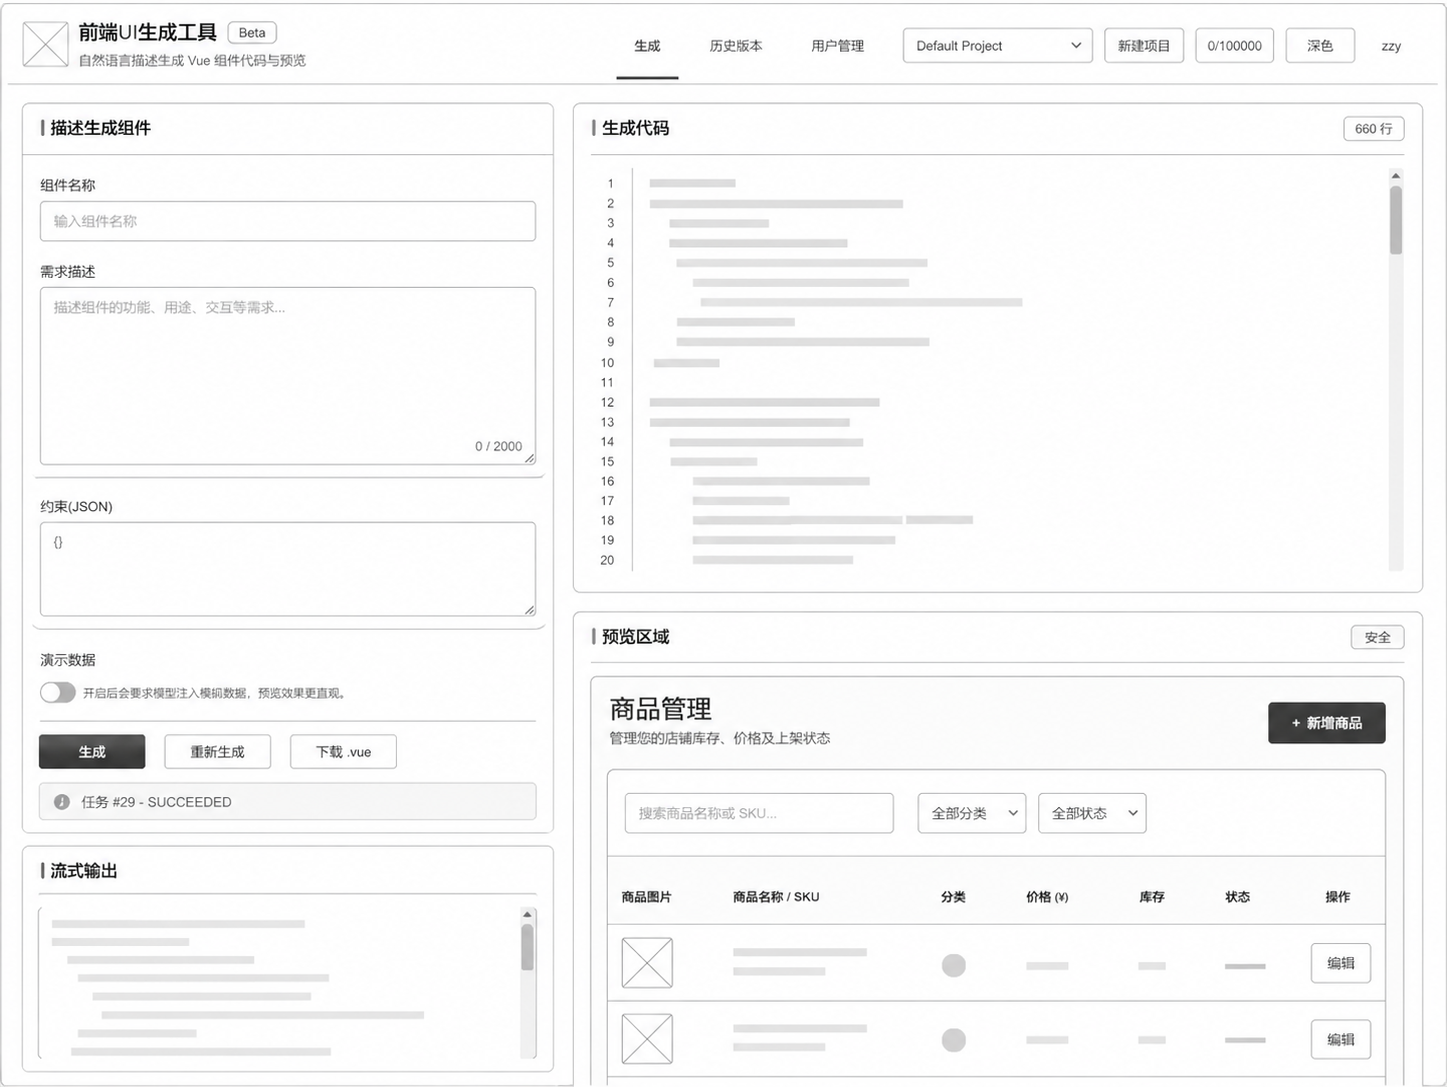
\includegraphics[width=0.96\textwidth,height=0.42\textheight,keepaspectratio]{figures/主界面原型图.png}
\caption{生成工作台线框图}
\label{fig:chapter4-wireframe-generator}
\end{figure}

除了生成工作台，登录注册页、历史版本页和用户管理页也构成了系统的主要使用路径。登录注册页负责建立身份状态，历史页负责回看与复用已有任务，用户管理页负责管理员治理。相关原型图分别见图 \ref{fig:chapter4-wireframe-login}、图 \ref{fig:chapter4-wireframe-history} 和图 \ref{fig:chapter4-wireframe-user-admin}。

\begin{figure}[!htbp]
\centering
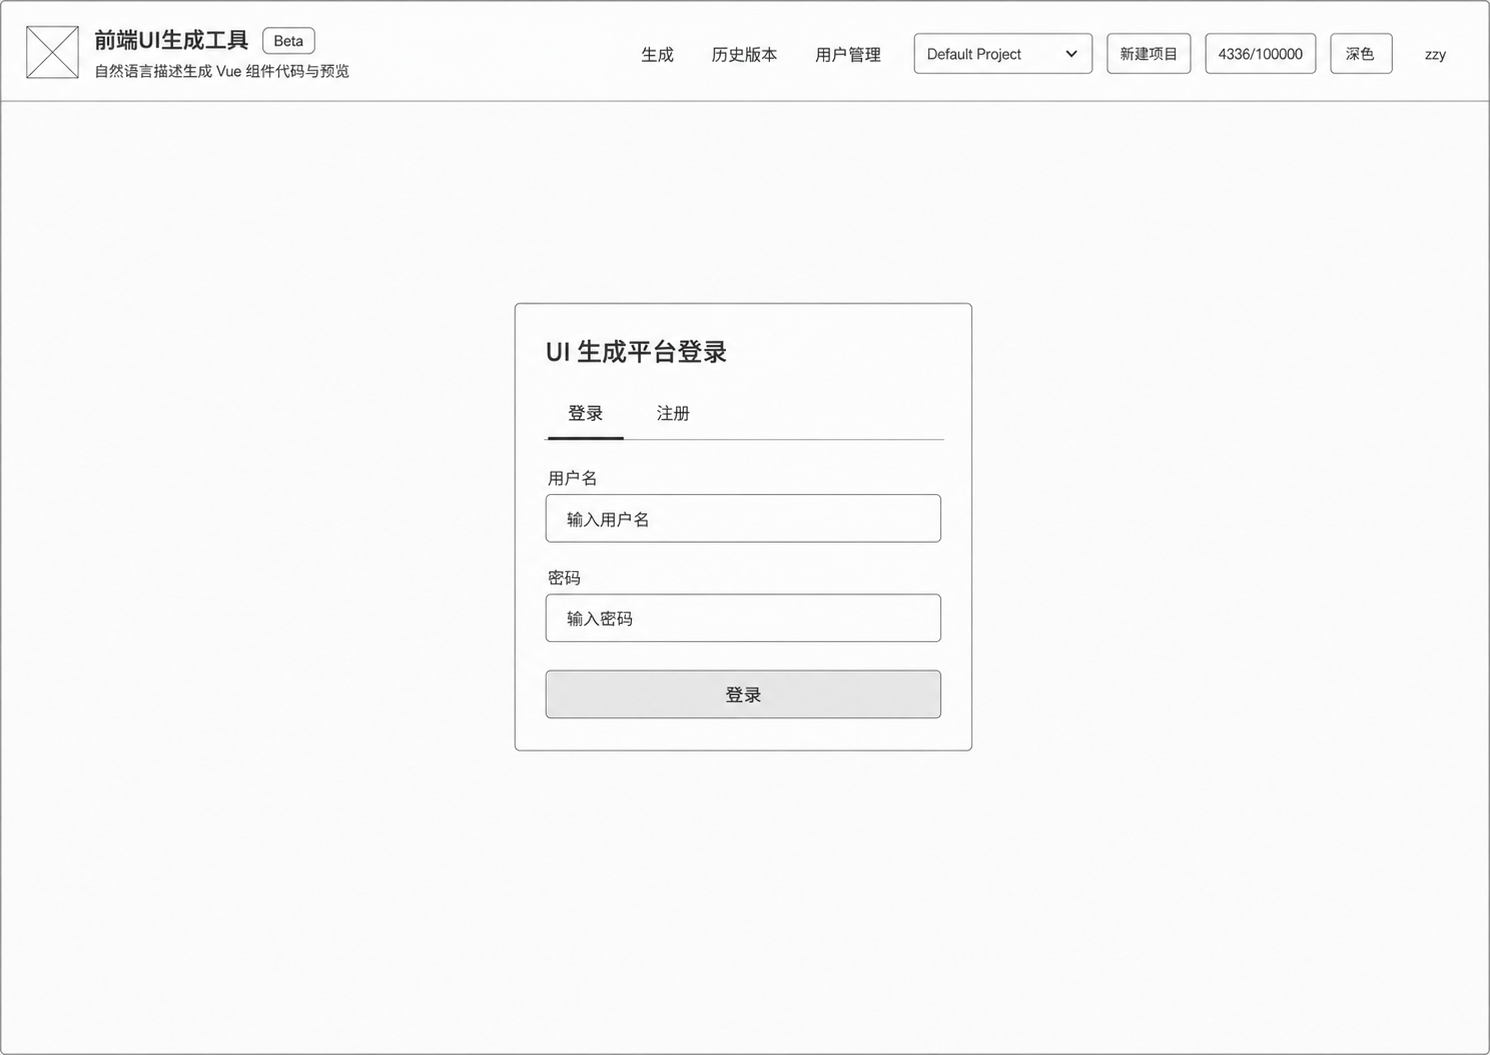
\includegraphics[width=0.72\textwidth,height=0.34\textheight,keepaspectratio]{figures/登录注册页面原型图.png}
\caption{登录注册页面线框图}
\label{fig:chapter4-wireframe-login}
\end{figure}

\begin{figure}[!htbp]
\centering
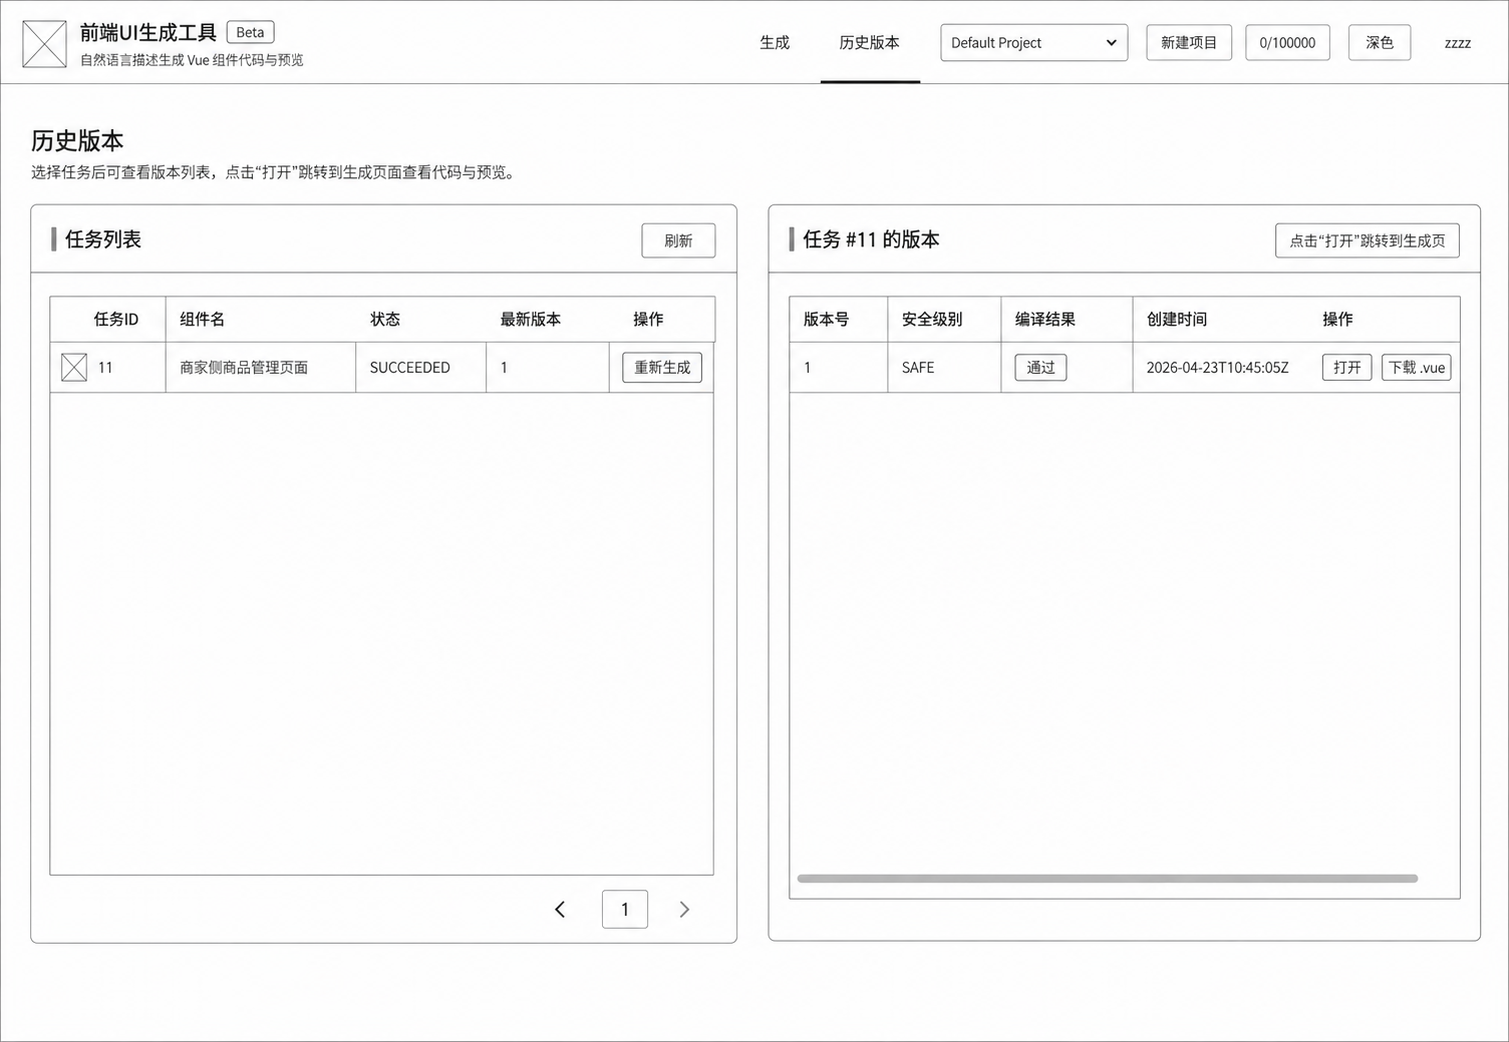
\includegraphics[width=0.96\textwidth,height=0.34\textheight,keepaspectratio]{figures/版本管理原型图.png}
\caption{历史版本页面线框图}
\label{fig:chapter4-wireframe-history}
\end{figure}

\begin{figure}[!htbp]
\centering
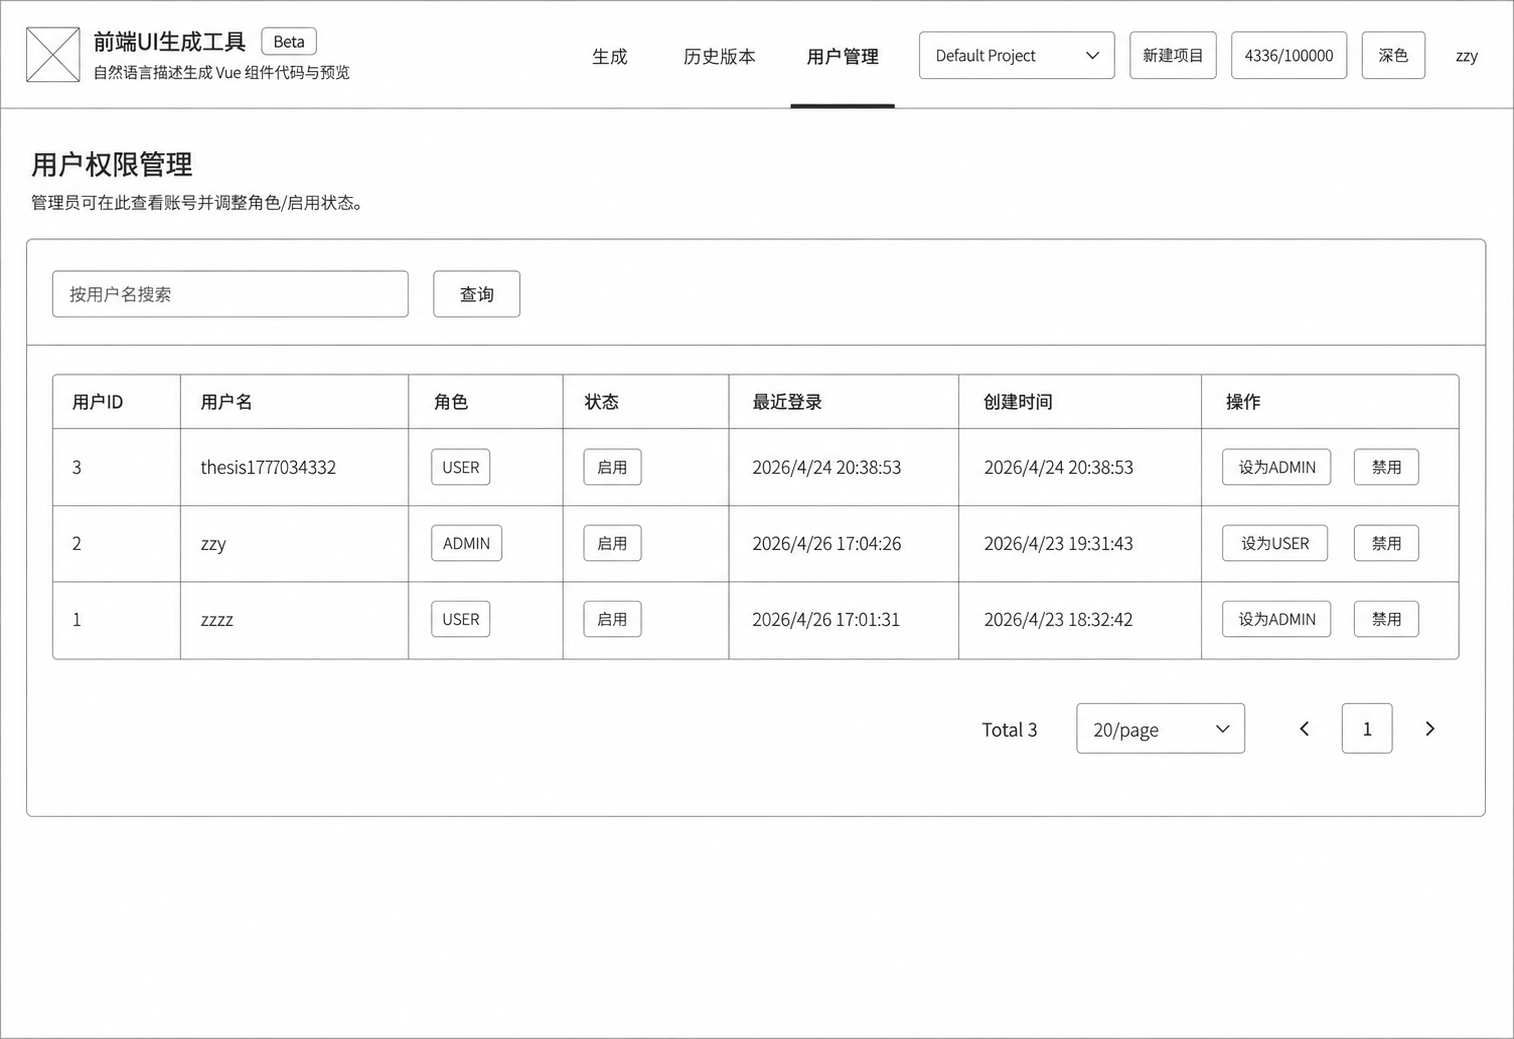
\includegraphics[width=0.96\textwidth,height=0.34\textheight,keepaspectratio]{figures/用户管理原型图.png}
\caption{用户管理页面线框图}
\label{fig:chapter4-wireframe-user-admin}
\end{figure}

登录注册页采用单卡片结构，将账号输入、登录入口和注册入口集中在同一界面中，以减少首次使用时的操作复杂度。历史版本页采用双列表布局，左侧定位任务，右侧查看版本，适合历史回看场景。用户管理页采用检索工具栏、数据表格和分页区组合，便于管理员快速完成筛选、角色调整和账号启停。这样的页面组织方式与当前前端代码中的路由划分和组件布局保持一致，也为下一章的系统实现说明提供了直接对应的界面基础。
